\documentclass{report}
\usepackage[T1]{fontenc} % Fontes T1
\usepackage[utf8]{inputenc} % Input UTF8
\usepackage[backend=biber, style=ieee]{biblatex} % para usar bibliografia
\usepackage{csquotes}
\usepackage[portuguese]{babel} %Usar língua inglesa
\usepackage{blindtext} % Gerar texto automáticamente
\usepackage[printonlyused]{acronym}
\usepackage{hyperref} % para autoref
\usepackage{graphicx}
\usepackage{listings}
        \usepackage{color}
        \definecolor{dkgreen}{rgb}{0,0.6,0}
        \definecolor{gray}{rgb}{0.5,0.5,0.5}
        \definecolor{mauve}{rgb}{0.8,0,0.82}
        \lstset{frame=tb, language=python, aboveskip=3mm, belowskip=3mm, showstringspaces=false, columns=flexible, basicstyle={\small\ttfamily}, numbers=none, numberstyle=\tiny\color{gray}, keywordstyle=\color{blue}, commentstyle=\color{dkgreen}, stringstyle=\color{mauve}, breaklines=true, breakatwhitespace=true, tabsize=3}

\bibliography{bibliografia}


\begin{document}
%%
% Definições
%
\def\titulo{PROJETO 2 - RELATÓRIO FINAL}
\def\data{5 de Junho de 2015}
\def\autores{Domingos Nunes, Dzianis Bartashevich, Francisco Cunha, Leonardo Oliveira}
\def\autorescontactos{dfsn@ua.pt, bartashevich@ua.pt, franciscomiguelcunha@ua.pt, leonardooliveira@ua.pt}
\def\versao{Versão 1.0}
\def\departamento{Departamento de Eletrónica, Telecomunicações e Informática}
\def\empresa{Universidade de Aveiro}
\def\logotipo{images/ua.pdf}
%
%% CAPA %%
%
\begin{titlepage}

\begin{center}
%
\vspace*{50mm}
%
{\Huge \titulo}\\ 
%
\vspace{10mm}
%
{\Large \empresa}\\
%
\vspace{10mm}
%
{\LARGE \autores}\\ 
%
%
\vspace{30mm}
%
\begin{figure}[h]
\center
\includegraphics{\logotipo}
\end{figure}
%
\vspace{20mm}
\end{center}
%
\begin{flushright}
\versao
\end{flushright}
\end{titlepage}

%
%
%%  Página de Título %%
%
%
\title{%
{\Huge\textbf{\titulo}}\\
{\Large \departamento\\ \empresa}
}
%
\author{%
    \autores \\
    \autorescontactos
}
%
\date{\data}
%
\maketitle
%%%%%%%%%%%%%%%%%%%%%%%%%%%%%%%%%%%%%%%%%%%
% RESUMO
%
%
\pagenumbering{roman}



\tableofcontents
\listoffigures


%%%%%%%%%%%%%%%%%%%%%%%%%%%%%%%
\clearpage
\pagenumbering{arabic}

%%%%%%%%%%%%%%%%%%%%%%%%%%%%%%%%
\chapter{Introdução}
\label{chap.introducao}
Este documento contém uma abordagem geral das etapas de realização do projeto 2 de Laboratórios de Informática, de acordo com o enunciado disponibilizado na plataforma \textit{moodle} da universidade \cite{moodle}.

Neste sentido, este documento está dividido em 7 capítulos. Depois desta introdução, no \autoref{chap.aplicacao} é apresentada a estrutura das páginas \ac{html} necessárias à interação com a aplicação, no \autoref{chap.servidor} são referidos alguns aspetos sobre o servidor, no \autoref{chap.som}, são tratados os módulos necessários ao processamento e geração de ficheiros de som e no \autoref{chap.base} é apresentada a árvore da base de dados a ser criada. Já no \autoref{chap.fases}, estão presentes as datas planeadas para o desenvolvimento do projeto, assim como a distribuição de tarefas da fase inicial. Finalmente, no \autoref{chap.finais} são apresentadas algumas considerações finais.

%%%%%%%%%%%%%%%%%%%%%%%%%%%%%%%%
\chapter{Aplicação Web}
\label{chap.aplicacao}

\section{Aplicação móvel}
A versão móvel da aplicação contém cinco páginas: introdutória, nova música, interpretação, playSong e About Us.

\subsection{Página Introdutória}
Nesta página (ver \autoref{intro}) faz-se uma introdução da aplicação móvel com uma ligação para entrar na página "nova música". Esta página é a única que não contém as barras fixas superior e inferior de navegação: na superior encontra-se o nome da página actual e um botão para regressar à pagina introdutória com atualização da aplicação móvel (lado direito). Finalmente, na barra inferior, temos disponíveis a ligações de interesse para as restantes páginas da aplicação móvel. (ver \autoref{music}, \autoref{inter}, \autoref{play} e \autoref{us}).

\begin{figure}[htp]
\centering
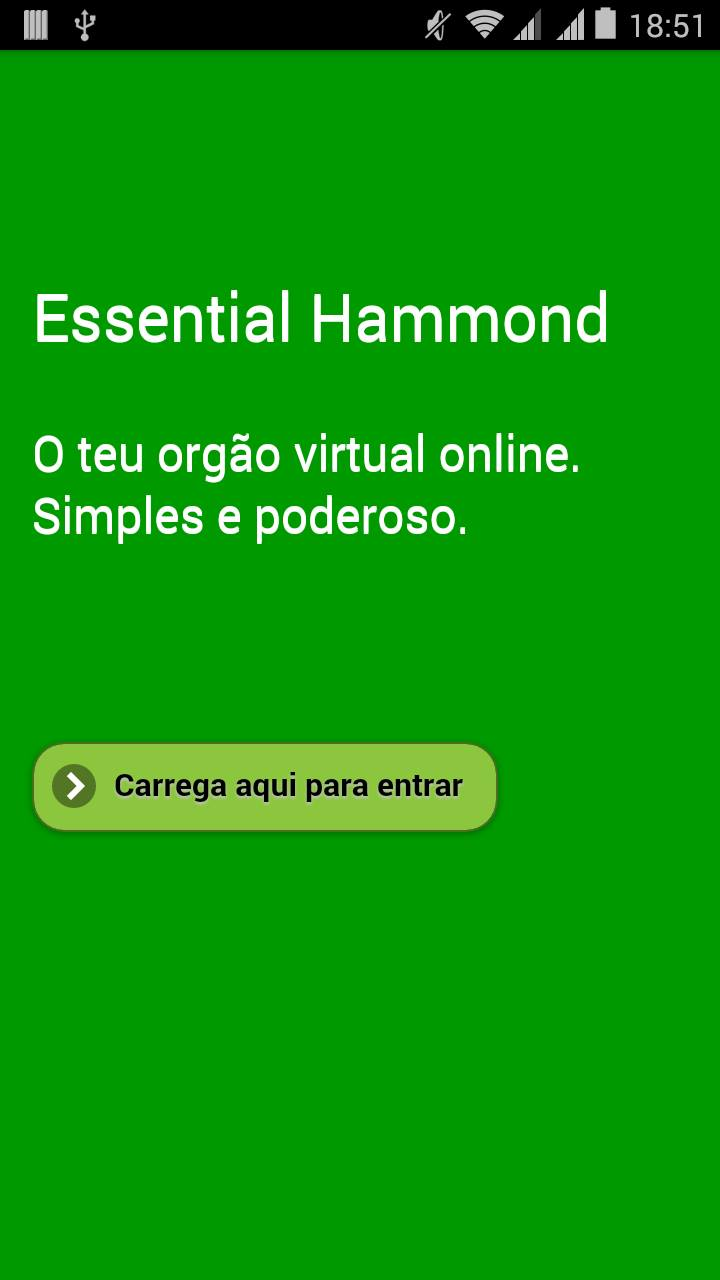
\includegraphics[width=50mm]{images/appIntro.jpg}
\caption{Página Introdutória da aplicação móvel.}
\label{intro}
\end{figure}

\subsection{Nova Música}
Nesta secção, o utilizador pode escrever as suas pautas na caixa de texto criada para o efeito e enviar para o servidor através de um botão (ver \autoref{music}). Quando o processamento é finalizado é enviado uma mensagem ao utilizador de acordo com o sucesso ou o insucesso do mesmo. 

\begin{figure}[htp]
\centering
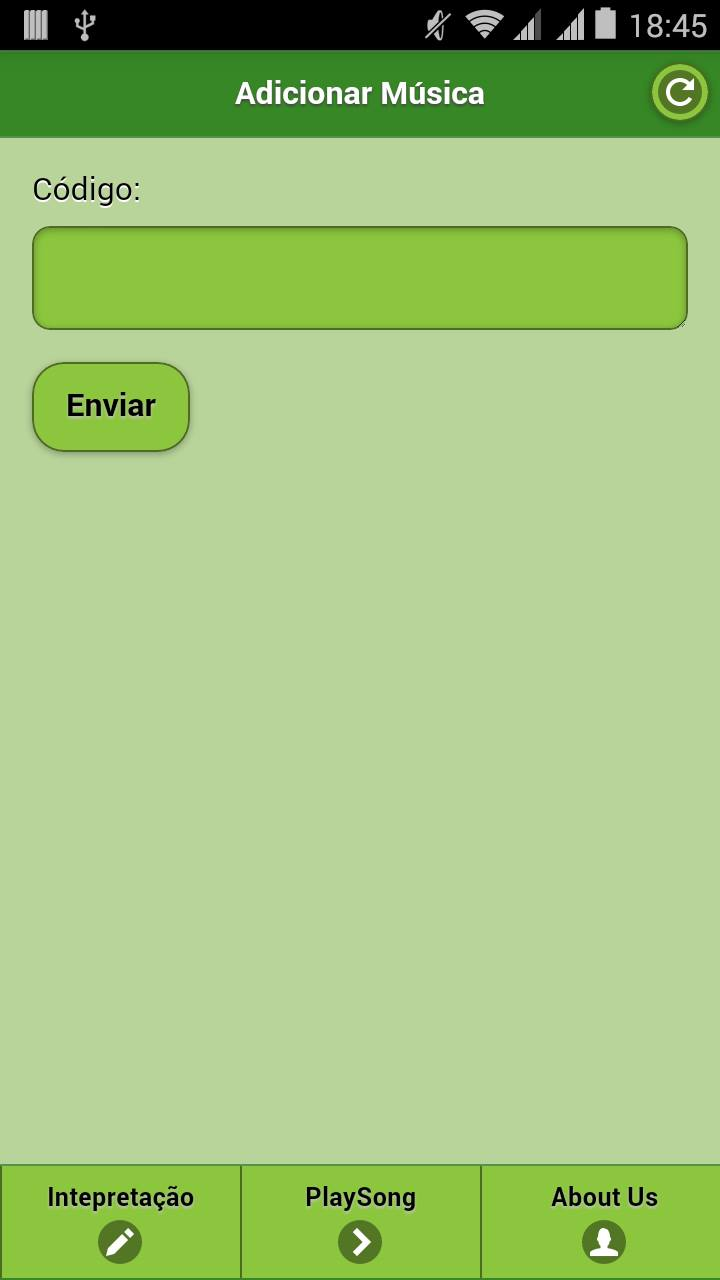
\includegraphics[width=50mm]{images/appAddNote.jpg}
\caption{Página de envio da música ao servidor.}
\label{music}
\end{figure}

\subsection{Interpertação}
Esta página corresponde ao último passo que o utilizador tem de dar para a criação do ficheiro audio. Para isso, ele tem de escolher a música, registo, efeito e o nome para o ficheiro, como podemos ver na figura \autoref{inter}. Como na página "Nova Música", o utilizador vai receber mensagens de aviso após o processamento do servidor.

\begin{figure}[htp]
\centering
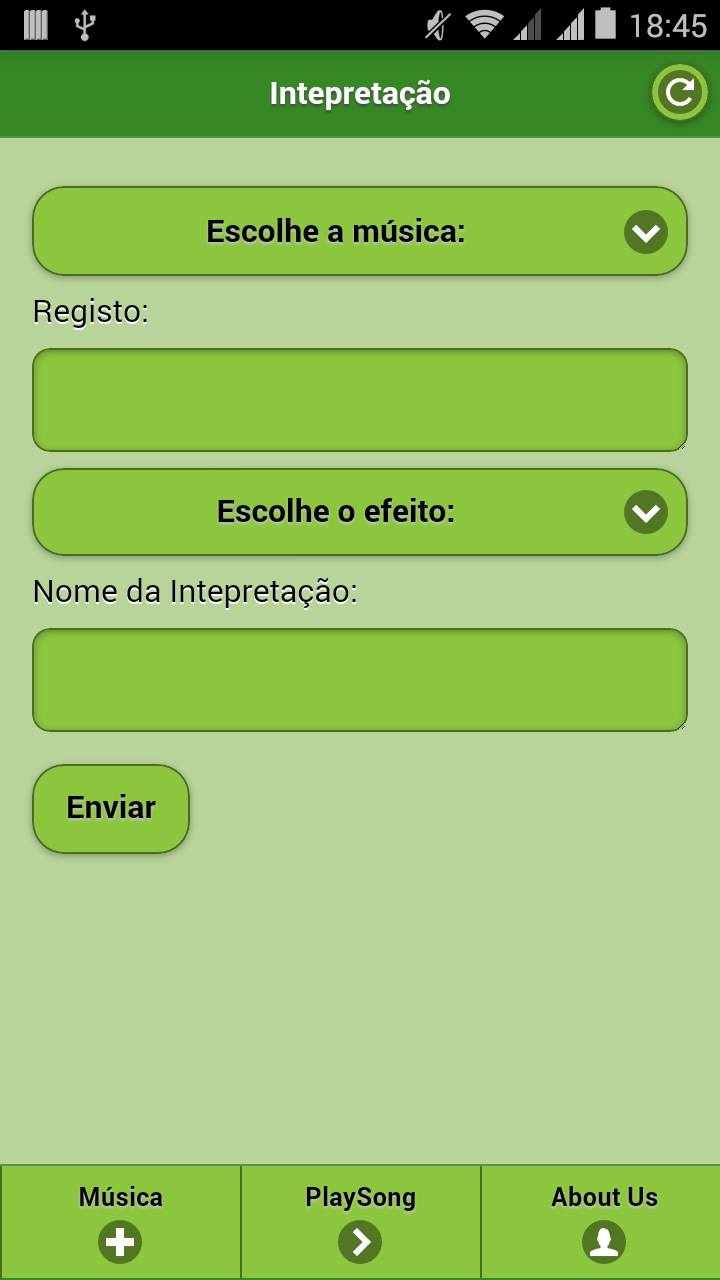
\includegraphics[width=50mm]{images/appAddMusic.jpg}
\caption{Página de envio da interpretação ao servidor.}
\label{inter}
\end{figure}

\subsection{PlaySong}

Inicialmente, nesta página, o utilizador tem disponível um \emph{pop-up} para escolher a música. Ao pressionar no botão "Procurar", a app móvel irá encontrar as interpretações que a musica anteriormente escolhida está associada e serão imediatamente visiveis. Cada interpretação irá conter um \emph{slidedown} individual com várias funcionalidades: contagem de gostos e não gostos, botões de gosto e não gosto, um botão "imagem" em que a imagem da pauta será visualizada através de um \emph{pop-up} e, finalmente, a reprodução audio da interpretação em questão (ver figura \autoref{play}).

\begin{figure}[htp]
\centering
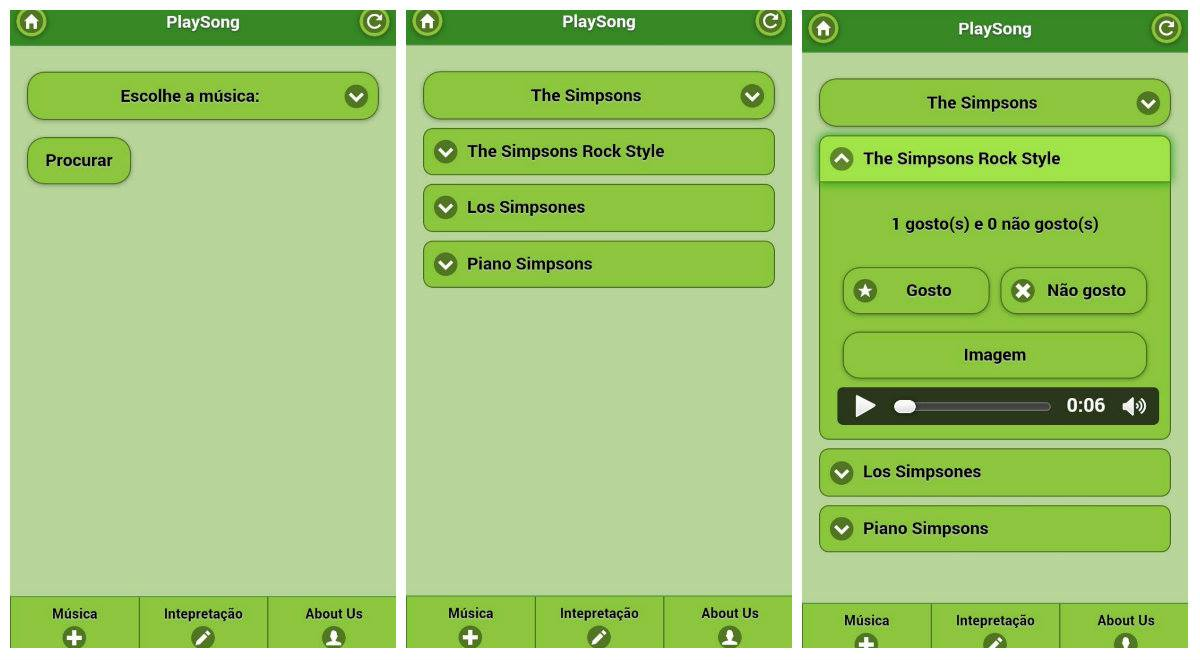
\includegraphics[width=\textwidth]{images/appPlaySong.jpg}
\caption{Página de reprodução das interpretações e mais algumas funcionalidades.}
\label{play}
\end{figure}

\subsection{About Us}

Nesta página, serão visualizados todos os alunos responsáveis pela a criação desta aplicação. Ao carregar num aluno abre-se um \emph{pop-up} contendo mais informações sobre o aluno, como a cidade, idade, curso e nº mecanográfico. (ver figura \autoref{us}).

\begin{figure}[htp]
\centering
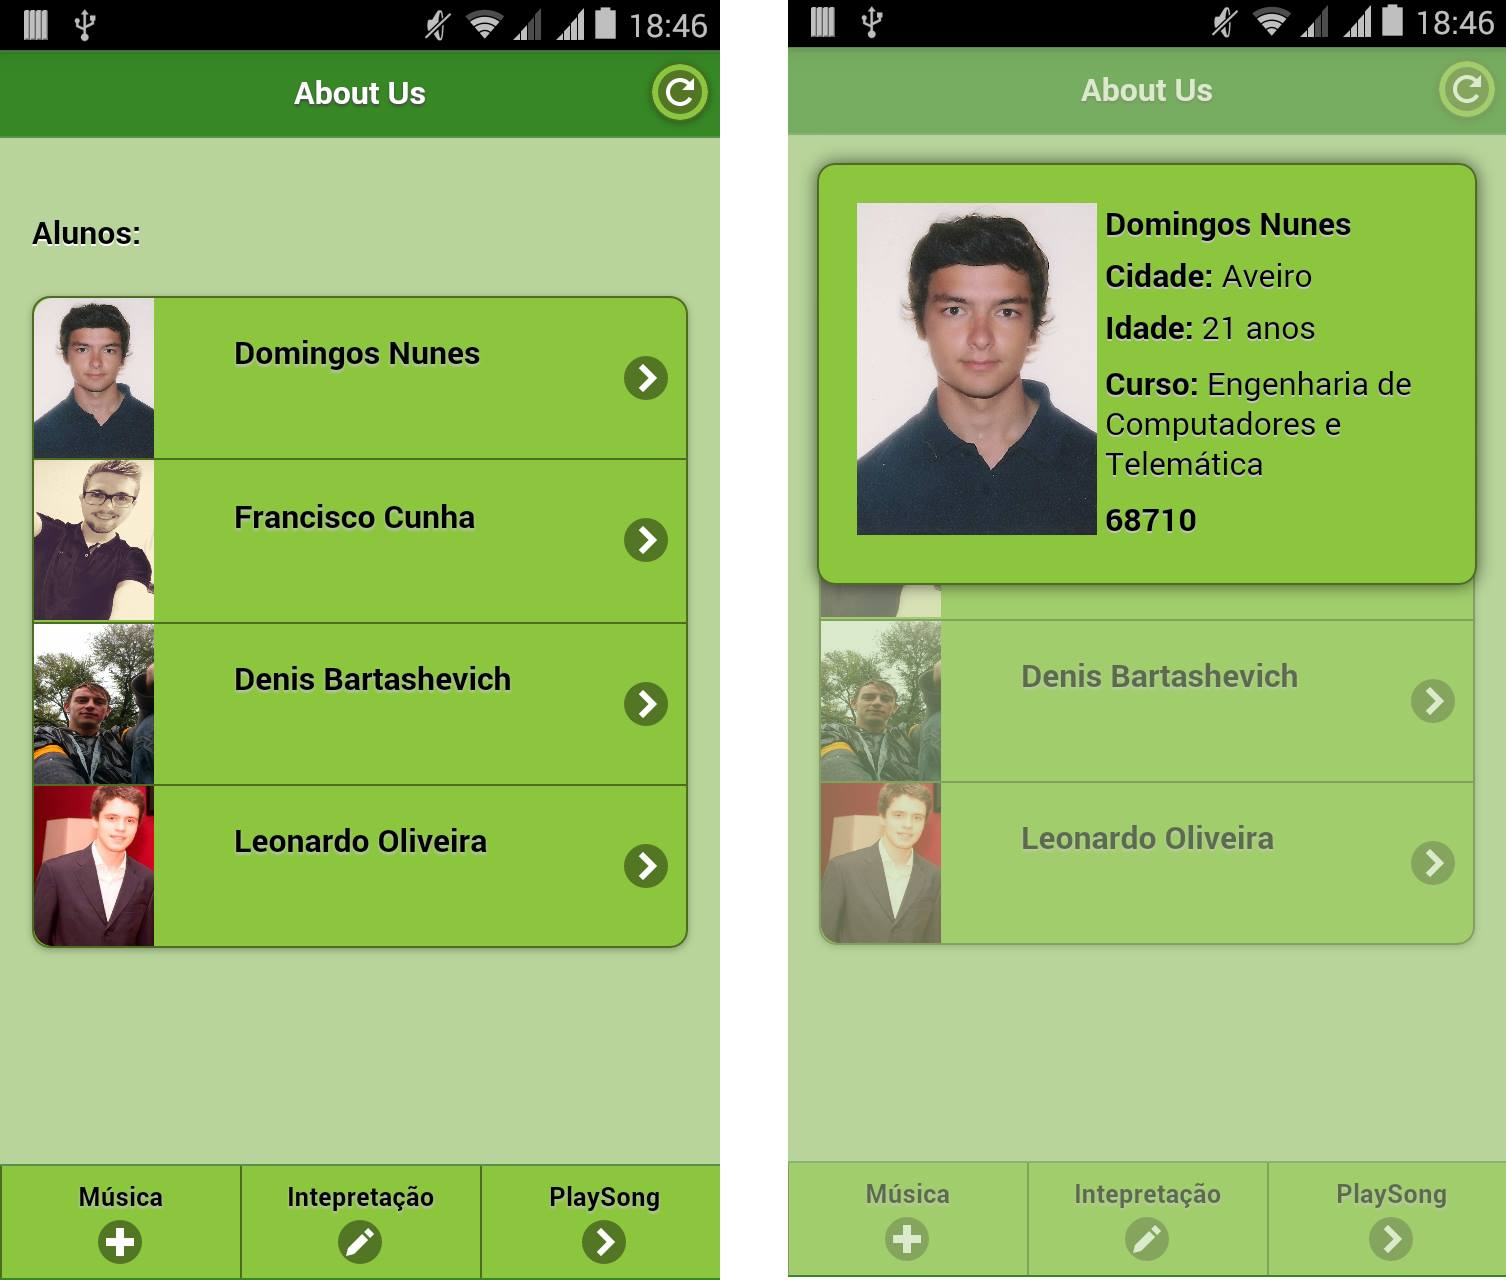
\includegraphics[width=\textwidth]{images/appUs.jpg}
\caption{Página sobre o grupo responsável por este trabalho.}
\label{us}
\end{figure}

\section{Aplicação Desktop}


\chapter{Servidor}
\label{chap.servidor}

O programa server.py for construído  com o módulo CherryPy \cite{cherry}. Fizemos as seguintes importações: cherrypy, sqlite3 e os.path. As restantes importações são programas construídos pelos membros do grupo: interpreter, synthesizer, effects\_processor e database.

O server.py possui uma única class (Root) onde se encontram os seguintes módulo criados: mobile, addVote, delVote, index, novainterpretacao, tocarmusica, sobrenos, createSong, createInterpretation, getWaveForm, getWaveFile, getNotes, listSongFiles, listNotes e listSongs.

\section{index, novamusica, novainterpretacao, tocarmusica}
Verifica se o website esta a ser acedido através de um dispositivo móvel ou computador. Caso seja móvel irá redirecionar sempre para o index da versão \emph{mobile}. Caso contrário, devolve a página pedida na versão \emph{desktop}.

\section{createSong}
Recebe como argumentos o nome e a pauta, verificando se estão minimamente válidos (nome não pode ser vazio, a pauta não pode estar vazia - quando o javascript envia notas vazias, o módulo recebe-as no formato undefined:undefined). Após a verificação é feita descodificação para \emph{String} dos parâmetros recebidos. Depois de converter é criada a imagem com o nome igual ao id das notas na tabela musics da base de dados. A criação de imagem também serve de metodo de verificação pois, se ocorrer algum erro na criação, uma exceção é lançada e o programa envia uma mensagem de erro. Caso a imagem seja criada com sucesso, os dados são enviados para base de dados e é devolvida uma mensagem de sucesso.

\section{createInterpretation}
Recebe como argumentos o registo, o id da pauta, o efeito e o nome, fazendo a verificação (registo tem de ser númerico, tamanho do registo só pode ser 9, o registo não pode conter o algarismo 9, nome não pode ser vazio, efeito não pode ser vazio, id não pode ser vazio, id tem de ser numérico). Antes de criar o ficheiro .wav é necessário ir buscar e juntar o nome e as notas do id fornecido como argumento. Caso na criação do ficheiro .wav ocorra uma exceção, o programa imprime uma mensagem de erro. Se o ficheiro for criado com sucesso, a informação sobre a interpretação (argumentos do módulo) irá ser guardada na base de dados e irá ser devolvida uma mensagem de sucesso.

\section{getWaveForm, getWaveFile}
Recebe como argumento o id da música/interpretação, que depois irá redirecionar para o ficheiro .jpg/.wav. Caso o ficheiro nao exista será lançada a excessão \emph{404NotFound}.

\section{getNotes}
Recebe como argumento o id da tabela musics, devolvendo as notas na forma de \emph{String}.

\section{listSongFiles}
Recebe como argumento o id da tabela musics, onde irá buscar todas as interpretações feitas sobre essa musica, retornando na forma de \ac{json}.

\section{listNotes, listSongs}
Não recebe nenhum argumento, devolvendo em formato \ac{json} todas as tabelas de musics (tablema das notas) / interpretations (tabela das interpretações), respetivamente.

Formato do json devolvido (listNotes):
\begin{lstlisting}
[
	{
		"notes": "d=4,o=5,b=160:c.6, e6, f#6, 8a6, g.6, e6, c6, 8a, 8f#, 8f#, 8f#, 2g, 8p, 8p, 8f#, 8f#, 8f#, 8g, a#., 8c6, 8c6, 8c6, c6",
		"id": 1,
		"name": "The Simpsons"
	}
]
\end{lstlisting}
Formato do json devolvido (listSongs) : 

\begin{lstlisting}
[
	{
		"name": "The Simpsons Rock Style",
		"id_music": 1,
		"downvotes": 10,
		"effects": "distortion",
		"registration": 888800000,
		"upvotes": 2,
		"id": 1
	}
]
\end{lstlisting}

\section{addVote, delVote}
Recebe como argumento o id da interpretação onde irá adicionar, na tabela interpretations, uma unidade ao campo upvote / downvote, respetivamente. Caso a interpretação não exista ou a operação não ocorra por outro motivo, devolve uma mensagem de erro.

\section{mobile}
(Para testes) Força a aparecer a versão \emph{mobile} do site, mesmo que o utilizador esteja a aceder a partir de um computador.

\chapter{Som}
\label{chap.som}

Os módulos ligados ao processamento e geração de ficheiros de som seguiram os moldes do que foi sugerido no enunciado do projeto. Foi criado um interpretador de pautas, um sintetizador e um processador de efeitos.

\section{Interpretador de pautas}

O interpretador recebe uma pauta no formato \ac{rtttl} e devolve uma lista de pares duração-frequência, cada par correspondendo à nota e a sua respetiva duração. Tomemos como exemplo a seguinte pauta:

\vspace{5mm}
\textbf{"Barbie girl : d=4, o=5, b=125 : 8g\#, 8e, 8g\#, 8c\#6, a, p, 8f\#, 8d\#, 8f\#, 8b, g\#, 8f\#, 8e, p, 8e, 8c\#, f\#, c\#, p, 8f\#, 8e, g\#, f\#'}
\vspace{5mm}

No caso desta pauta, o interpretador devolve uma lista com 23 pares, com a seguinte estrutura:

\vspace{5mm}
\begin{lstlisting}
[{'freq': 830, 'time': 0.24}, {'freq': 659, 'time': 0.24}, {'freq': 830, 'time': 0.24}, {'freq': 1108, 'time': 0.24} ... ]
\end{lstlisting}
\vspace{5mm}

Internamente, o interpretador começa por ignorar a primeira parte da pauta, correspondente ao nome. De seguida, analiza os valores dos parâmetros de referência, d, o e b. Caso algum não esteja definido, é aplicado o valor padrão (d=4, o=6 e b=63). Por fim, extrai a parte correspondente às notas e percorre nota a nota, tendo a vírgula como refeencia para as separar. Para determinar a frequência da nota para uma dada oitava, foi criada uma \emph{lookup table}, sendo devolvida a frequência quando é inserido como parâmetro a seguinte expressão: [12 * oitava + tom] - com a oitava a variar entre 0 e 7 e o tom entre 0 e 11, sendo o 0 correspondente ao dó e o 11 ao si. No final do cálculo da frequência e tempo de cada nota, o par é adicionado à lista, que no final é devolvida.

\section{Sintetizador}
O sintetizador recebe como argumentos os pares vindos do interpretador e um registo, devolvendo uma nova lista com a frequência (principal) e respetivas amostras ao processador de efeitos. Inicialmente são criadas as seguintes variáveis:

\begin{itemize}
\item Uma lista vazia, que irá ser a devolvida no final;
\item Uma lista de tamanho 9, que irá conter os 9 frequências para cada nota;
\item Uma lista de tamanho 9 com os múltiplos para o cálculo das 9 frequências para cada nota, de acordo com os osciladores: [1/2, 2/3, 1, 2, 3, 4, 5, 6, 8];
\item Uma lista de tamanho 9 que irá conter as amplitudes das frequências para cada nota, de acordo com os valores definidos no registo.
\item Um inteiro para a frequência de amostragem, que é sempre 44100.
\end{itemize}

De seguida, o sintetizador percorre a lista de pares recebido do interpretador, alterando a lista de frequências para cada nota. Para casa par produz as amostras com a duração definida, correspondendo à soma das 9 componentes sinosoidais. Estas têm a amplitude e frequência previamente calculadas e guardadas nas listas referidas acima. No final de cada nota ser processada, a frequência principal e amostras são adicionadas à lista que no final vai ser devolvida. A lista fica com a seguinte estrutura:

\vspace{5mm}
\begin{lstlisting}
[{"freq": 830, "samples": [0, 11775, 18804, 19193, 14747, 9339, ...], {"freq": 659, "samples": [...], ...]
\end{lstlisting}
\vspace{5mm}

Os cuidados com a possível existência de clipping não são tomados nesta altura, pelo ue existirá um método para normalizar as amostras mais à frente, no processador de efeitos.

\section{Processador de efeitos}
O processador de efeitos recebe a lista de sons vinda do sintetizador e o efeito pretendido, tendo ccomo função gerar o ficheiro de som da música. Nas secções seguintes irá ser explicado como é aplicado cada um dos efeitos.

\subsection{Efeito nulo}
A partir da lista de sons fornecida, extrai a lista de samples de cada som e junta-os numa única lista, para poder

\subsection{Efeito eco}
Aplica inicialmente o efeito nulo e, seguidamente, percorre a lista de amostras, somando a cada uma um múltiplo (inferior a 1, para atenuar) da amostra correspondente a 0,1 segundos atrás e outro múltiplo (mais pequeno que o anterior, para atenuar ainda mais, pois é um eco mais atrasado) da amostra 0,2 segundos atrás. Deste modo, são introduzidos dois ecos, com atrasos de 0,1 e 0,2 segundos.

\subsection{Efeito trémolo}
Aplica inicialmente o efeito nulo e, seguidamente, percorre a lista de amostras, elevando ao quadrado cada amostra.

\subsection{Efeito distorção}

\subsection{Efeito percurssão}

\subsection{Efeito coro}

\subsection{Efeito envelope}


Depois do efeito pretendido ser aplicado, as amostras são normalizadas, para poderem estar contidas no intervalo de resolução (-32768 to 32767), sendo posteriormente empacotadas e utilizadas na geração do ficheiro wav.


\chapter{Base de dados}
\label{chap.base}

A base de dados associada a este projecto são duas tabelas \textbf{musics, interpretations} que estão interligadas entre si e as quais servirão para armazenar informação acerca dos conteúdos.

A tabela \textbf{musics} conterá informação com o \textbf{name} das músicas criadas e as \textbf{notes} (pautas) que lhes são correspondentes, sendo que a estes dois campos há um \textbf{id} que os identifica.

Por outro lado, a tabela \textbf{interpretation} terá campos como:

\textbf{\texttt{id\_music}} que estará associado à tabela \textbf{musics}. Conterá também campos como \textbf{(registration)} (registos) que servirá para a codificação do registo  e o campo \textbf{effects} (efeitos), servindo para guardar informação sobre e os efeitos utilizados na música.
Finalmente, os campos \textbf{upvotes} e \textbf{downvotes} guardarão respectivamente o número de votos positivos e negativos.

A \autoref{tree} apresenta o esquema da árvore da base de dados.

\begin{figure}[htp]
\centering
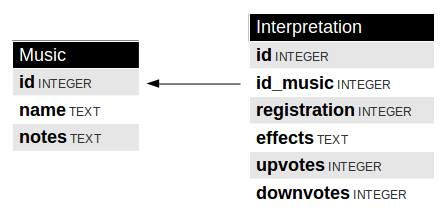
\includegraphics[width=\textwidth]{images/tree.jpg}
\caption{Árvore da base de dados, com as tabelas da música (\emph{musics}) e interpretação (\emph{interpretation}).}
\label{tree}
\end{figure}

Dentro do ficheiro que cria a base de dados, há uma condição que verifica se se encontra criada a base de dados, ou então se é o próprio programa que a cria, através do ficheiro \emph{create.txt}.

\vspace{5mm}
\begin{lstlisting}
if not os.path.isfile('songs.db'):
	
	if not os.path.isfile('create.txt'):
		print 'We need a database to run the program. We don\'t have one, so we need a "create.txt" file to create the library. Copy a valid "create.txt" file to this folder and reopen the program.'
		exit(1)
		
	db = sql.connect('songs.db')
	
	createDBfile = open('create.txt', 'r')
	
	for line in createDBfile:
		db.execute(line)	
	
	db.commit()
	createDBfile.close()
	db.close()
\end{lstlisting}
\vspace{5mm}

Dentro do próprio programa, existe uma série de funções que permite efectuar operações na base de dados.

\vspace{5mm}
\begin{lstlisting}
def is_mobile(request):
    ismobile = False

    if request.headers.has_key('User-Agent'):
        user_agent = request.headers['User-Agent']

        # Test common mobile values.
        patterns = "(xoom|up.browser|up.link|mmp|symbian|smartphone|phone|tablet|midp|wap|windows ce|pda|mobile|mini|palm|netfront|nokia)"

        patt_compiled = re.compile(patterns, re.IGNORECASE)
        match = patt_compiled.search(user_agent)

        if match:
           ismobile = True

    return ismobile
\end{lstlisting}
\vspace{5mm}

Esta função, permite que a base de dados ao comunicar com o servidor, permite saber se o dispositivo onde vai ser executado a aplicação é um dispositivo móvel ou um computador, sendo depois mostrado ao utilizador a interface correspondente.  

\vspace{5mm}
\begin{lstlisting}
def create_song(name, notes):
	command = 'INSERT INTO musics(name, notes) VALUES("' + name + '", "' + notes + '")'
	db.execute(command)
	db.commit()
\end{lstlisting}
\vspace{5mm}

A função acima descrita permite criar uma nova música na tabela das músicas, sendo que a cada nova música adicionada irá haver uma \textbf{id} que lhes é atribuida, facilitando desta forma identificar a música mais facilmete caso seja necessário fazer alterações. Para criar uma nova interpretação seguem-se os mesmos padrões do exemplo anterior.

Tal como é possível adicionar novas músicas, também se pode visualizar o conteúdo de uma tabela, neste caso, o conteúdo da \textbf{interpretations}, através do exemplo seguinte:

\vspace{5mm}
\begin{lstlisting}
def get_all_notes():
	command = 'SELECT * FROM musics'
	result = db.execute(command)
	rows = result.fetchall()
	d = []
	for row in rows:
		name = {"id":row[0],"name":row[1],"notes":row[2]}
		d.append(name)

	return d
\end{lstlisting}
\vspace{5mm}

Para ser possível actualizar o número de votos, neste caso positivos, sendo o mesmo método aplicado no número de gostos negativos, recorreu-se ao seguinte código. Esta função vai mostrar os votos positivos de uma determinada interpretação, sendo o valor guardado numa variável onde será incrementado em mais uma unidade. Após isso executa-se um novo comando e actualiza-se o número de gostos positivos para o novo valor.  

\vspace{5mm}
\begin{lstlisting}
def add_upvotes(ID):
	command = 'SELECT upvotes FROM interpretations WHERE id = ' + str(ID)
	result = db.execute(command)
	result = result.fetchone()
	result = result[0] + 1
	command = 'UPDATE interpretations SET upvotes = "' + str(result) + '" WHERE id = ' + str(ID)
	db.execute(command)
	db.commit()

\end{lstlisting}
\vspace{5mm}


\vspace{5mm}
\begin{lstlisting}

def last_id_interpretations():
	try:
		result = db.execute("SELECT id FROM interpretations")
		rows = result.fetchall()
		x = []
		for row in rows:
			x.append(row[0])

		return x[len(x)-1]+1
	except IndexError, e:
		return 1

\end{lstlisting}

Como se pode verificar pelo código acima descrito, esta função vai tentar apanhar uma exceção, quando mostra todas as \textbf{id's} da tabela interpretações, guardando-as numa lista, verificando se a sequência está dentro do intervalo, e caso não esteja, a exceção é gerada. 

%%%%%%%%%%%%%%%%%%%%%%%%%%%%%%%%

\chapter{Fases de desenvolvimento}
\label{chap.fases}
Estão previstas três fases de desenvolvimento do projeto:

\begin{itemize}
\item Fase 1 - 13 de Maio a 21 de Maio (a decorrer);
\item Fase 2 - 22 de Maio a 29 de Maio;
\item Fase 3 - 30 de Maio a 7 de Junho.
\end{itemize}

\section{Fase 1}
Inicialmente, será desenvolvida cada uma das partes da aplicação em separado e a distribuição das tarefas é a seguinte:
\begin{itemize}
\item Domingos - Implementação do \textit{mockup} das páginas \ac{html};
\item Dzianis - Implementação do servido;
\item Francisco - Implementação da base de dados;
\item Leonardo - Implementação do sintetizador e interpretador de pautas.
\end{itemize}
\section{Fase 2}
Neste fase a aplicação será testada no seu todo, sendo efetuados os ajustes necessários ao seu correto funcionamento, podendo ser acrescentadas algumas funcionalidades úteis que não tenham sido previstas.
\section{Fase 3}
Finalmente, serão afetuados os ajustes finais, sendo também completado o módulo processador de efeitos, para que este comece efetivamente a criar efeitos nas músicas: Echo, Tremolo, Distorção, Percursão, Chorus e Envelope.

%%%%%%%%%%%%%%%%%%%%%%%%%%%%%%%%
\chapter{Considerações finais}
\label{chap.finais}

...


%%%%%%%%%%%%%%%%%%%%%%%%%%%%%%%%%
\chapter*{Acrónimos}
\begin{acronym}
\acro{sql}[SQL] {Structured Query Language}
\acro{html} [HTML] {HyperText Markup Language}
\acro{rtttl} [RTTTL] {Ring Tone Transfer Language}
\acro{json} [JSON] {JavaScript Object Notation}

\end{acronym}


%%%%%%%%%%%%%%%%%%%%%%%%%%%%%%%%%
\printbibliography

\end{document}